\documentclass[10pt, conference, a4paper, final]{IEEEtran}
\IEEEoverridecommandlockouts
\usepackage{amsmath, amssymb}
\usepackage[margin=1in]{geometry} % Adjust margins if needed
\usepackage{graphicx} % Required for including images
\usepackage{subcaption}
\usepackage{algorithm, algorithmicx} % For algorithms
\usepackage[table,xcdraw]{xcolor} % For colored tables
\usepackage{enumitem} % For better control over list
\usepackage{microtype} % Improves typography
\usepackage{amsmath}

% Combine graphicx package loading
\usepackage{float}
\usepackage{booktabs} % For professional looking tables

\title{ A Novel Testing Framework for Vision Models Using Bayesian Network}
\author{Author Name}
\date{\today}

\begin{document}

\maketitle

\begin{abstract}

    Deep learning models, particularly vision models (VMs), are critical in high-stake domains such as autonomous driving, medical diagnostics, and security systems. The real-world deployment of VMs require rigorous robustness testing due to diverse environmental conditions. Current testing approaches primarily focus on neuron coverage. Although this metric is critical; however, it alone does not ensure comprehensive coverage of all corner cases, which can lead to unexpected failures, thus leaving a gap in the overall evaluation of the VMs robustness. My research develops a comprehensive testing framework designed to enhance the evaluation of VMs through a structured five-stage process.
    The initial stage, Specification Module, focuses on clearly defining all necessary properties of the system to guide the entire testing process and ensure comprehensive coverage. The second stage, Sampling, involves to gather all relevant samples necessary for thorough model testing. In the third stage, Test Case Generation, the properties are specified in the first stage are applied to the collected samples, and test cases are generated accordingly. For example, in autonomous car testing, properties such as dust, noise, rain, and night conditions are considered to evaluate model performance under these conditions. The fourth stage, Testing \& Probabilistic Graph, begins with testing the generated test cases to validate their effectiveness. After testing,  robustness assessments are conducted both locally and globally. Locally, the robustness of model is evaluated within individual categories or classes to identify weaknesses. In contrast, globally, the model’s performance is assessed across various categories to enhance its generalization capabilities across different scenarios. Errors are systematically recorded for later analysis. This stage integrates a probabilistic approach using Bayesian network, combined with solid mathematical formulation, to provide a comprehensive visual and quantitative analysis of the model’s performance at both local and global levels. The final stage, Error Summarization, compiles and analyses the recorded errors, producing actionable graphical error reports and recommendations for VMs refinement.
\end{abstract}


\section{Introduction}

\section{Problem Statement}

Deep learning models are being more widely used in a variety of applications, yet their reliability in practical applications remains a challenge.


\section{Research Goal}
This paper aims to develop a systematic framework for evaluating local and global robustness in deep learning models. 
The goal is to provide a comprehensive error summary to improve model design and training, ensuring their reliability for real-world applications.

\section{Contributions}
This research makes the following key contributions to the field of deep learning robustness evaluation:
\begin{itemize}
   
    \item We design an \textbf{end-to-end pipeline} for evaluating the robustness of system.
    
    \item We propose a \textbf{conceptual framework} that quantifies both local and global robustness,with formalized approach to verify system robustness.
    \item A novel \textbf{error summarization}  approach which allows better identification of model weaknesses related to class and property.

    \item We perform all our \textbf{experiments} using publicly available deep learning models and MNIST dataset.
\end{itemize}

\section{Research Questions}

This paper addresses the following research questions applicable to various deep learning models and datasets:

\begin{itemize}
    \item How can we design a comprehensive framework to test system robustness?
    \item How can we systematically evaluated the robustness both at local (property-specific) and global (overall system) levels within framework?
    \item How can error summarization be employed to quantify the impacts on model robustness?
 
\end{itemize}


\section{Methodology}
\begin{figure}{}
    \centering
    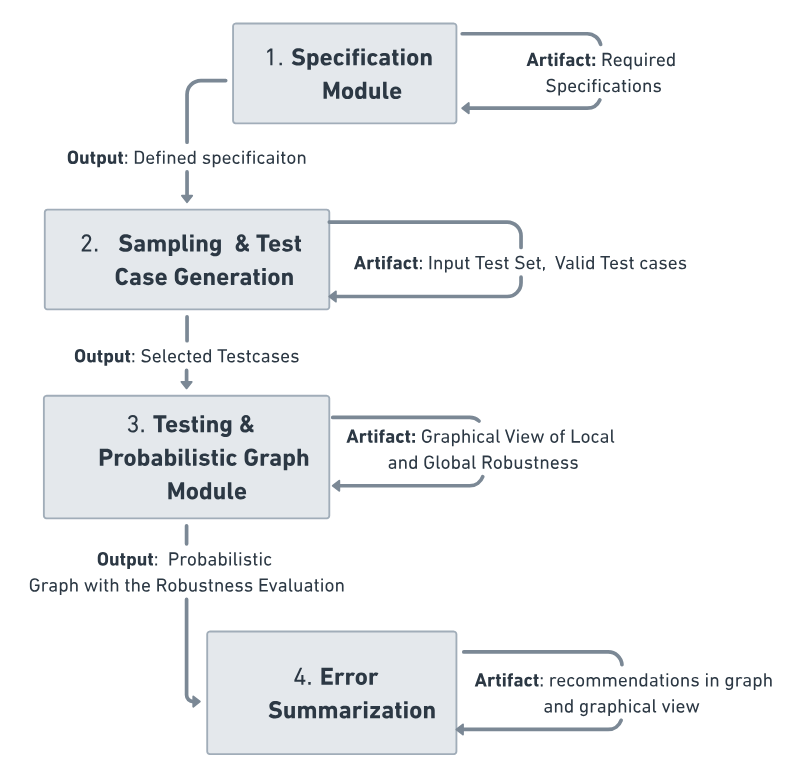
\includegraphics[width=\linewidth]{paper_images/framework.png}
    \caption{Overview of Testing Framework}
    \label{fig:graph}
\end{figure}


This section presents an overview of the comprehensive testing framework, which is intended to test the specified properties according to given specification. The pipeline begins by precisely describing the properties to be evaluated. To comprehensively examine the model, test cases are created and tested. The error summary step next concentrating on the progression from local to global robustness to highlight the system systemic strengths and weaknesses. This systematic technique improves the robustness of deep learning models by tackling each essential aspect sequentially, from specification to complete error analysis.

\subsection{Sampling}
 The sample selection process involves a random but balanced choice of samples from each class, focusing exclusively on instances that the model has correctly predicted. This method ensures a representative and fair distribution of data across all classes.

\begin{itemize}

    
        \item Model Utilization:
            \begin{itemize}
                \item A pre-trained CNN model is utilized to select samples.
                \item Let \( X = \{x_1, x_2, \dots, x_N\} \) denote the set of MNIST images. The model function \( f \) predicts:
                \[ f(x_i) \rightarrow y_i \]
                \item The filter function \( g \) identifies accurate predictions, defined as:
                \[ g(x_i) = 
                \begin{cases} 
                1 & \text{if } f(x_i) = \text{true label of } x_i \\
                0 & \text{otherwise}
                \end{cases} \]
                \item The subset \( S \) includes only correctly predicted images:
                \[ S = \{x_i \in X \mid g(x_i) = 1\} \]
            \end{itemize}
        \item Random Selection of Samples:
            \begin{itemize}
                \item Randomly selects 200 samples from each class in \( S \), totaling 2000 samples.
                \item The random selection function \( R \) is defined to ensure:
                \[ R(S_c, 200) \text{ for each class } c \text{ in } S \]
                where \( S_c \) represents the samples of class \( c \) within \( S \).
            \end{itemize}

\end{itemize}


\subsection{Test Case Generation}

This section outlines the generation of test cases to assess model robustness through properties such as noise, rotation, and brightness adjustments.

\begin{figure}{}
    \centering
    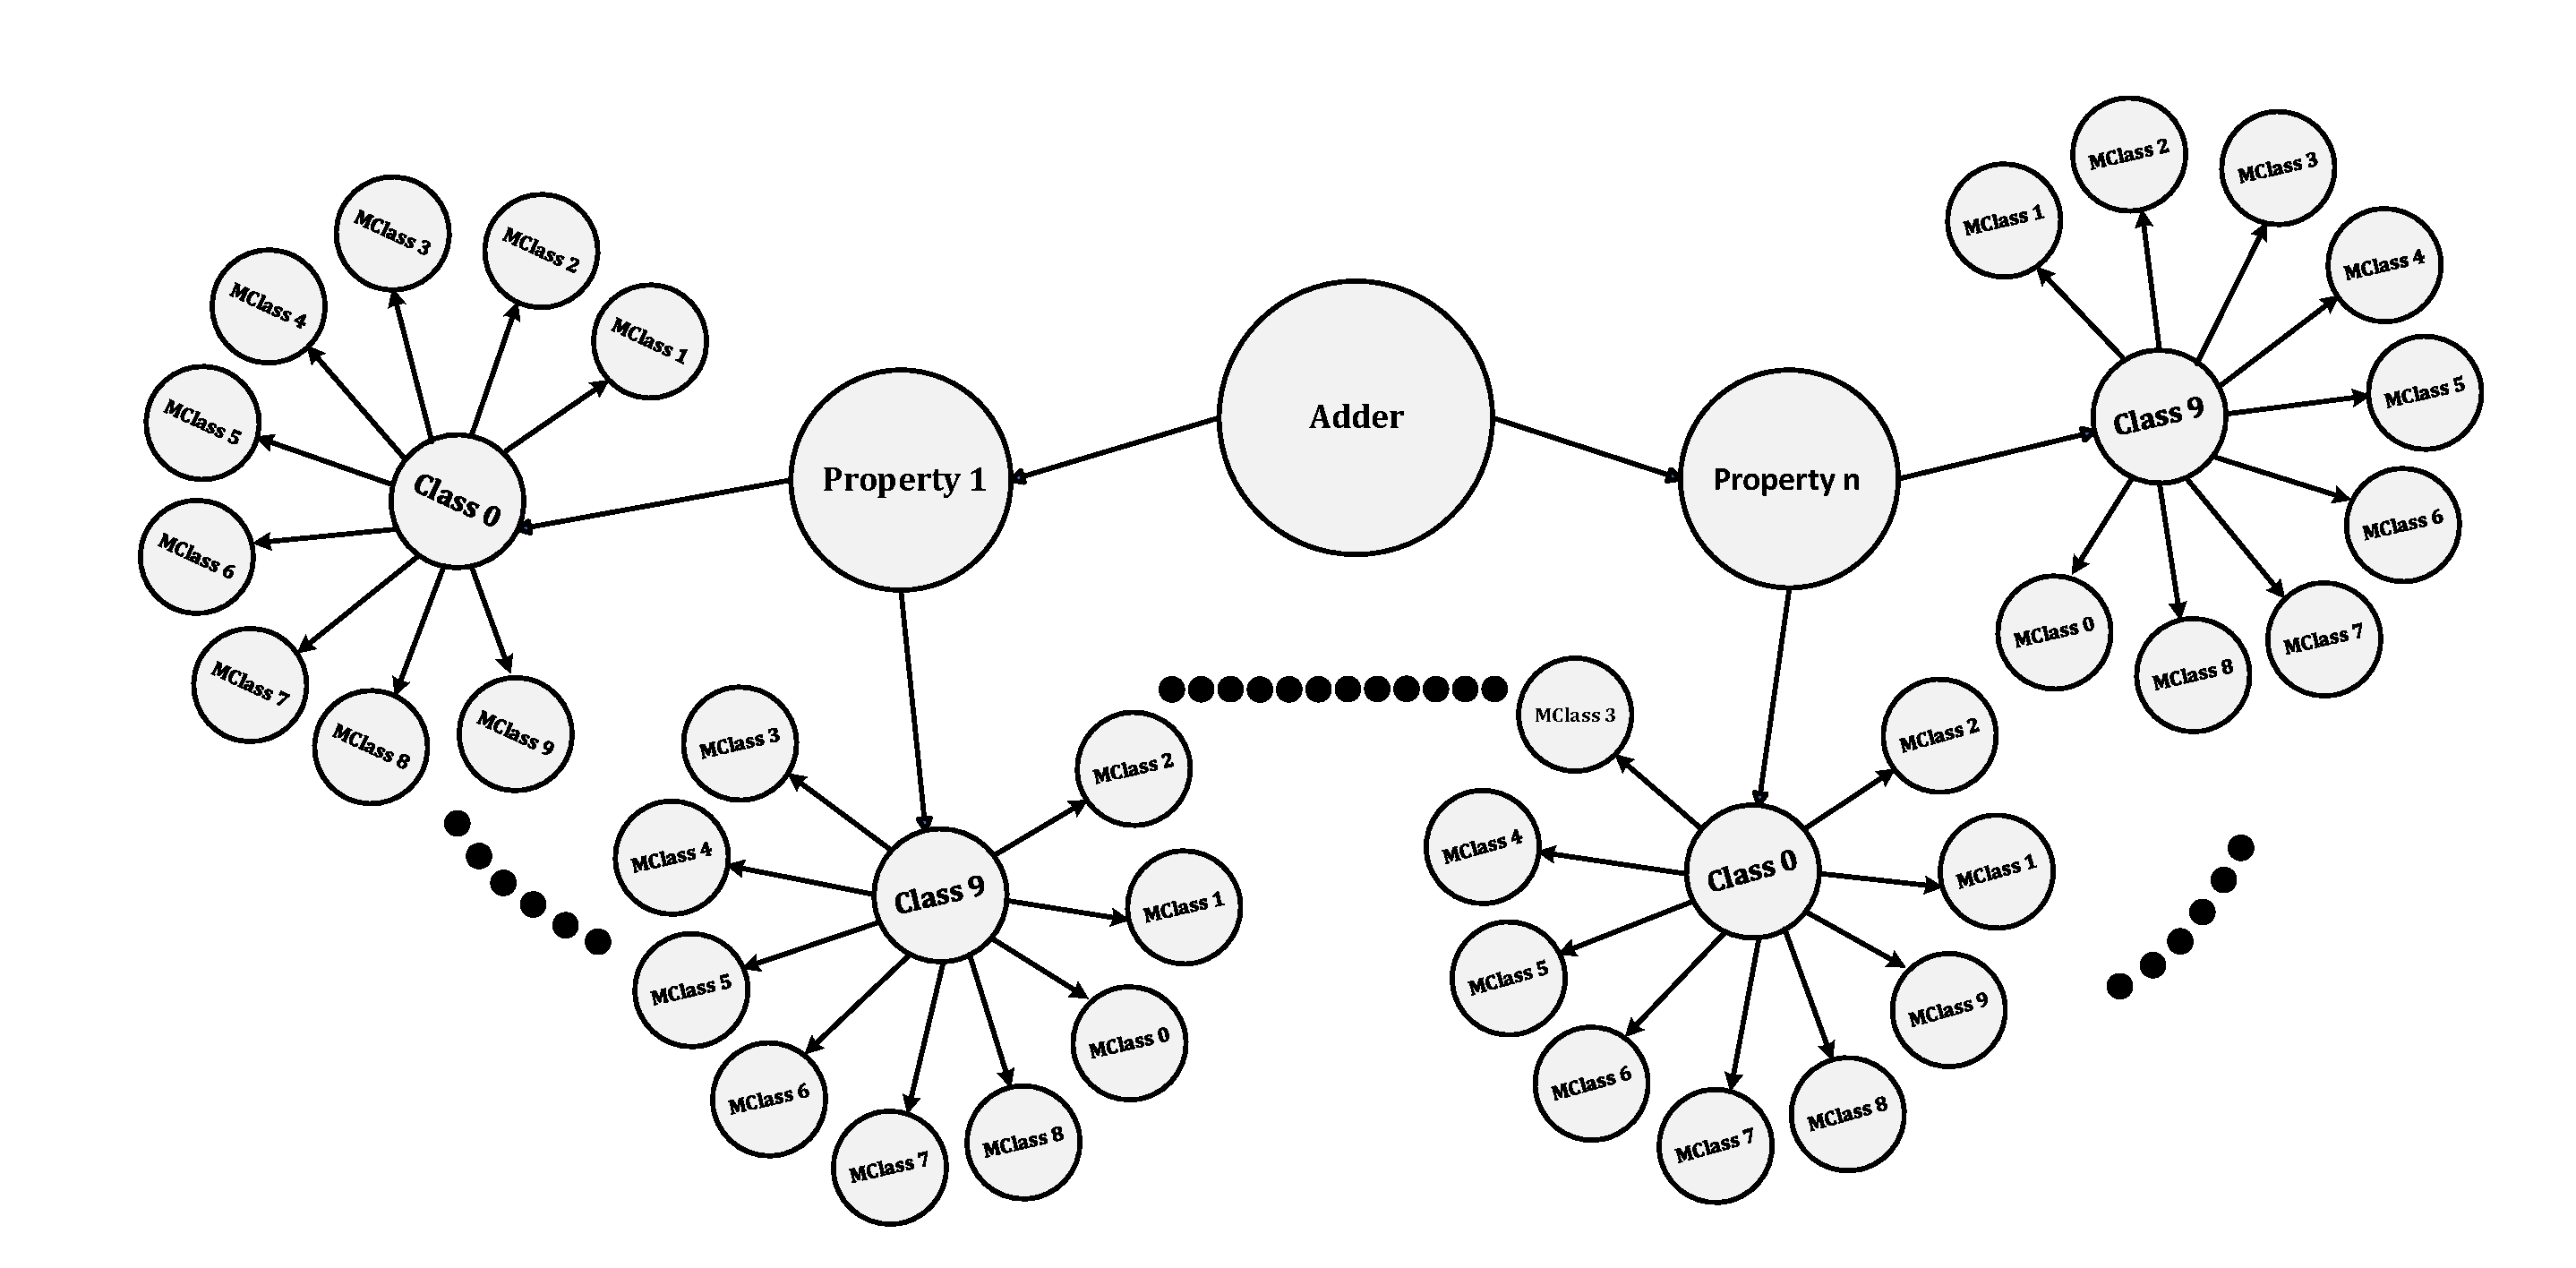
\includegraphics[width=\linewidth]{paper_images/step4.pdf}
    \caption{Graphical View of Local and Global Robustness}
    \label{fig:graph}
\end{figure}

\begin{itemize}
    \item \textbf{Noise Addition:} Noise is added to an image \( x_i \) using a Gaussian noise model. The noise function \( p_n \) is defined as:
    \[ p_n(x_i, \sigma) = x_i + \epsilon \]
    where \( \epsilon \sim \mathcal{N}(0, \sigma^2) \) denotes the Gaussian noise with mean zero and standard deviation \(\sigma\).

    \item \textbf{Rotation:} The rotation of an image \( x_i \) by an angle \(\theta\) is modeled by the rotation function \( p_r \):
    \[ p_r(x_i, \theta) = \text{rotate}(x_i, \theta) \]
    where \(\text{rotate}(\cdot, \theta)\) represents the rotation operation.

    \item \textbf{Brightness Adjustment:} Brightness adjustment of an image \( x_i \) is controlled by a multiplicative factor \( \beta \), which scales the intensity of all pixels. The brightness function \( p_b \) can be defined as:
    \[ p_b(x_i, \beta) = \beta \cdot x_i \]
    where \( \beta > 1 \) increases brightness, and \( \beta < 1 \) decreases it. This approach ensures that the image's contrast is preserved while adjusting its brightness.

\end{itemize}

\subsection{Testing }

The Testing section evaluates how accurately and confidently the model predicts under various properties (noise, rotation, brightness) applied to images from each class. This phase focuses on directly measuring and quantifying the robustness of the model.
\begin{itemize}

    \item Confidence Level Assessment:
        \begin{itemize}
            \item After generating test cases, measure the model’s confidence for each class under each type of property.
            \item Aggregate these measurements to assess the overall robustness of individual properties (noise, rotation, brightness).
        \end{itemize}

    \end{itemize}


    \subsection{Introduction to Local Robustness}
    Local robustness  assesses how consistent a model's predictions are when faced with alterations such as noise, rotation, and brightness adjustments. 
    \subsubsection{Definition}
    Local robustness for a class \(c\) subjected to a property \(p\) is formally defined as the conditional probability of the model correctly classifying a perturbed input:
    \begin{equation}
        LR_{c,p} = P(\hat{Y}_{c,p} = Y_c \mid X_c = x'_{c,p}),
    \end{equation}
    where \(X_c = x'_{c,p}\) denotes the input from class \(c\) modified by property \(p\), such as adding Gaussian noise or altering brightness.
    
    
    \subsubsection{Empirical Estimation}
    To measure local robustness in practice, the model is subjected to a series of tests involving perturbed inputs. The robustness is then quantified by averaging the outcomes of these tests:
    \begin{equation}
        \hat{LR}_{c,p} = \frac{1}{N} \sum_{i=1}^N \mathbf{1}(f(p(x_{c,i}, \theta_p)) = y_{c,i}),
    \end{equation}
    where \(N\) represents the number of test cases, and \(\mathbf{1}\) is the indicator function, which is 1 if the prediction is correct and 0 otherwise. 

    \subsubsection{Aggregation of Robustness Measures}
    While individual measures of local robustness are insightful, aggregating these metrics across different properties and classes provides a comprehensive view of the model's overall stability and reliability. For instance, averaging the robustness scores across all classes for a specific property can highlight how well the model handles that property in general:
    \begin{equation}
        LR_p = \frac{1}{C} \sum_{c=1}^C LR_{c,p},
    \end{equation}
    where \(C\) is the total number of classes. This aggregated metric helps in identifying properties that might require further optimization to enhance the model's overall performance.



        \subsection{Global Robustness Evaluation}
        Global robustness in this context evaluates the model's ability to process and synthesize outputs from multiple inputs, each subjected to the same type of perturbation, directly within an integrated adder function. This adder not only generates predictions but also combines them, assessing the collective output against a predefined combined result.
        
        \subsubsection{Definition and Integrated Functionality}
        The global robustness is defined with respect to an adder function that both predicts and combines outputs from two perturbed inputs:
        \begin{multline}
            GR_{(c1, c2), p} = P(\text{Adder}(x'_{c1,p}, x'_{c2,p}) = \\
            Y_{\text{combined}} \mid X_{c1} = x'_{c1,p}, X_{c2} = x'_{c2,p})
        \end{multline}
        where:        
        - \(x'_{c1,p}\) and \(x'_{c2,p}\) are the inputs from classes \(c1\) and \(c2\), respectively, after the application of property \(p\).
        - The \(\text{Adder}\) function now encapsulates the prediction process for each input and the subsequent combination of these predictions.
        - \(Y_{\text{combined}}\) is the expected result of this combination, reflecting the correct combined output for the inputs processed together.
        
        Empirical estimation of global robustness now involves:
        \begin{equation}
            \hat{GR} = \frac{1}{M} \sum_{j=1}^M \mathbf{1}(\text{Adder}(x'_{j1,p}, x'_{j2,p}) = Y_{j,\text{combined}})
        \end{equation}
        where:
        - \(M\) is the number of test pairs.
        - \(\mathbf{1}\) is the indicator function, returning 1 if the combined output from the adder matches the expected result, and 0 otherwise.
        - The \(\text{Adder}\) function within each test pair handles the prediction from perturbed inputs and their aggregation, effectively simulating a real-world application where input data are integrated to form a single decision output.
   
\subsection{Error Summarization}
This section details the error summarization process following the global robustness testing, where we identify and analyze discrepancies in the model's predictions. By tracing errors from the combined outputs back to individual properties and classes, we systematically pinpoint and address underlying weaknesses.

\subsubsection{Example Setup}
We consider two classes from the MNIST dataset:
\begin{itemize}
    \item Class A: Digit `5'
    \item Class B: Digit `0'
\end{itemize}
Both classes are tested under the properties of noise and rotation, with the following local robustness confidence levels:
\begin{itemize}
    \item \( LR_{A,p_1} = 85\% \) (Noise)
    \item \( LR_{A,p_2} = 78\% \) (Rotation)
    \item \( LR_{B,p_1} = 90\% \) (Noise)
    \item \( LR_{B,p_2} = 88\% \) (Rotation)
\end{itemize}

\subsubsection{Global Robustness Testing Scenario}
The model is tasked with processing two images, one from each class, both subjected to noise. The ideal prediction should reflect the sum `5' (Class A) + `0' (Class B) = `5'. An incorrect sum indicates a prediction error.

\subsubsection{Error Summarization Process}

\begin{figure}[H]
    \centering
    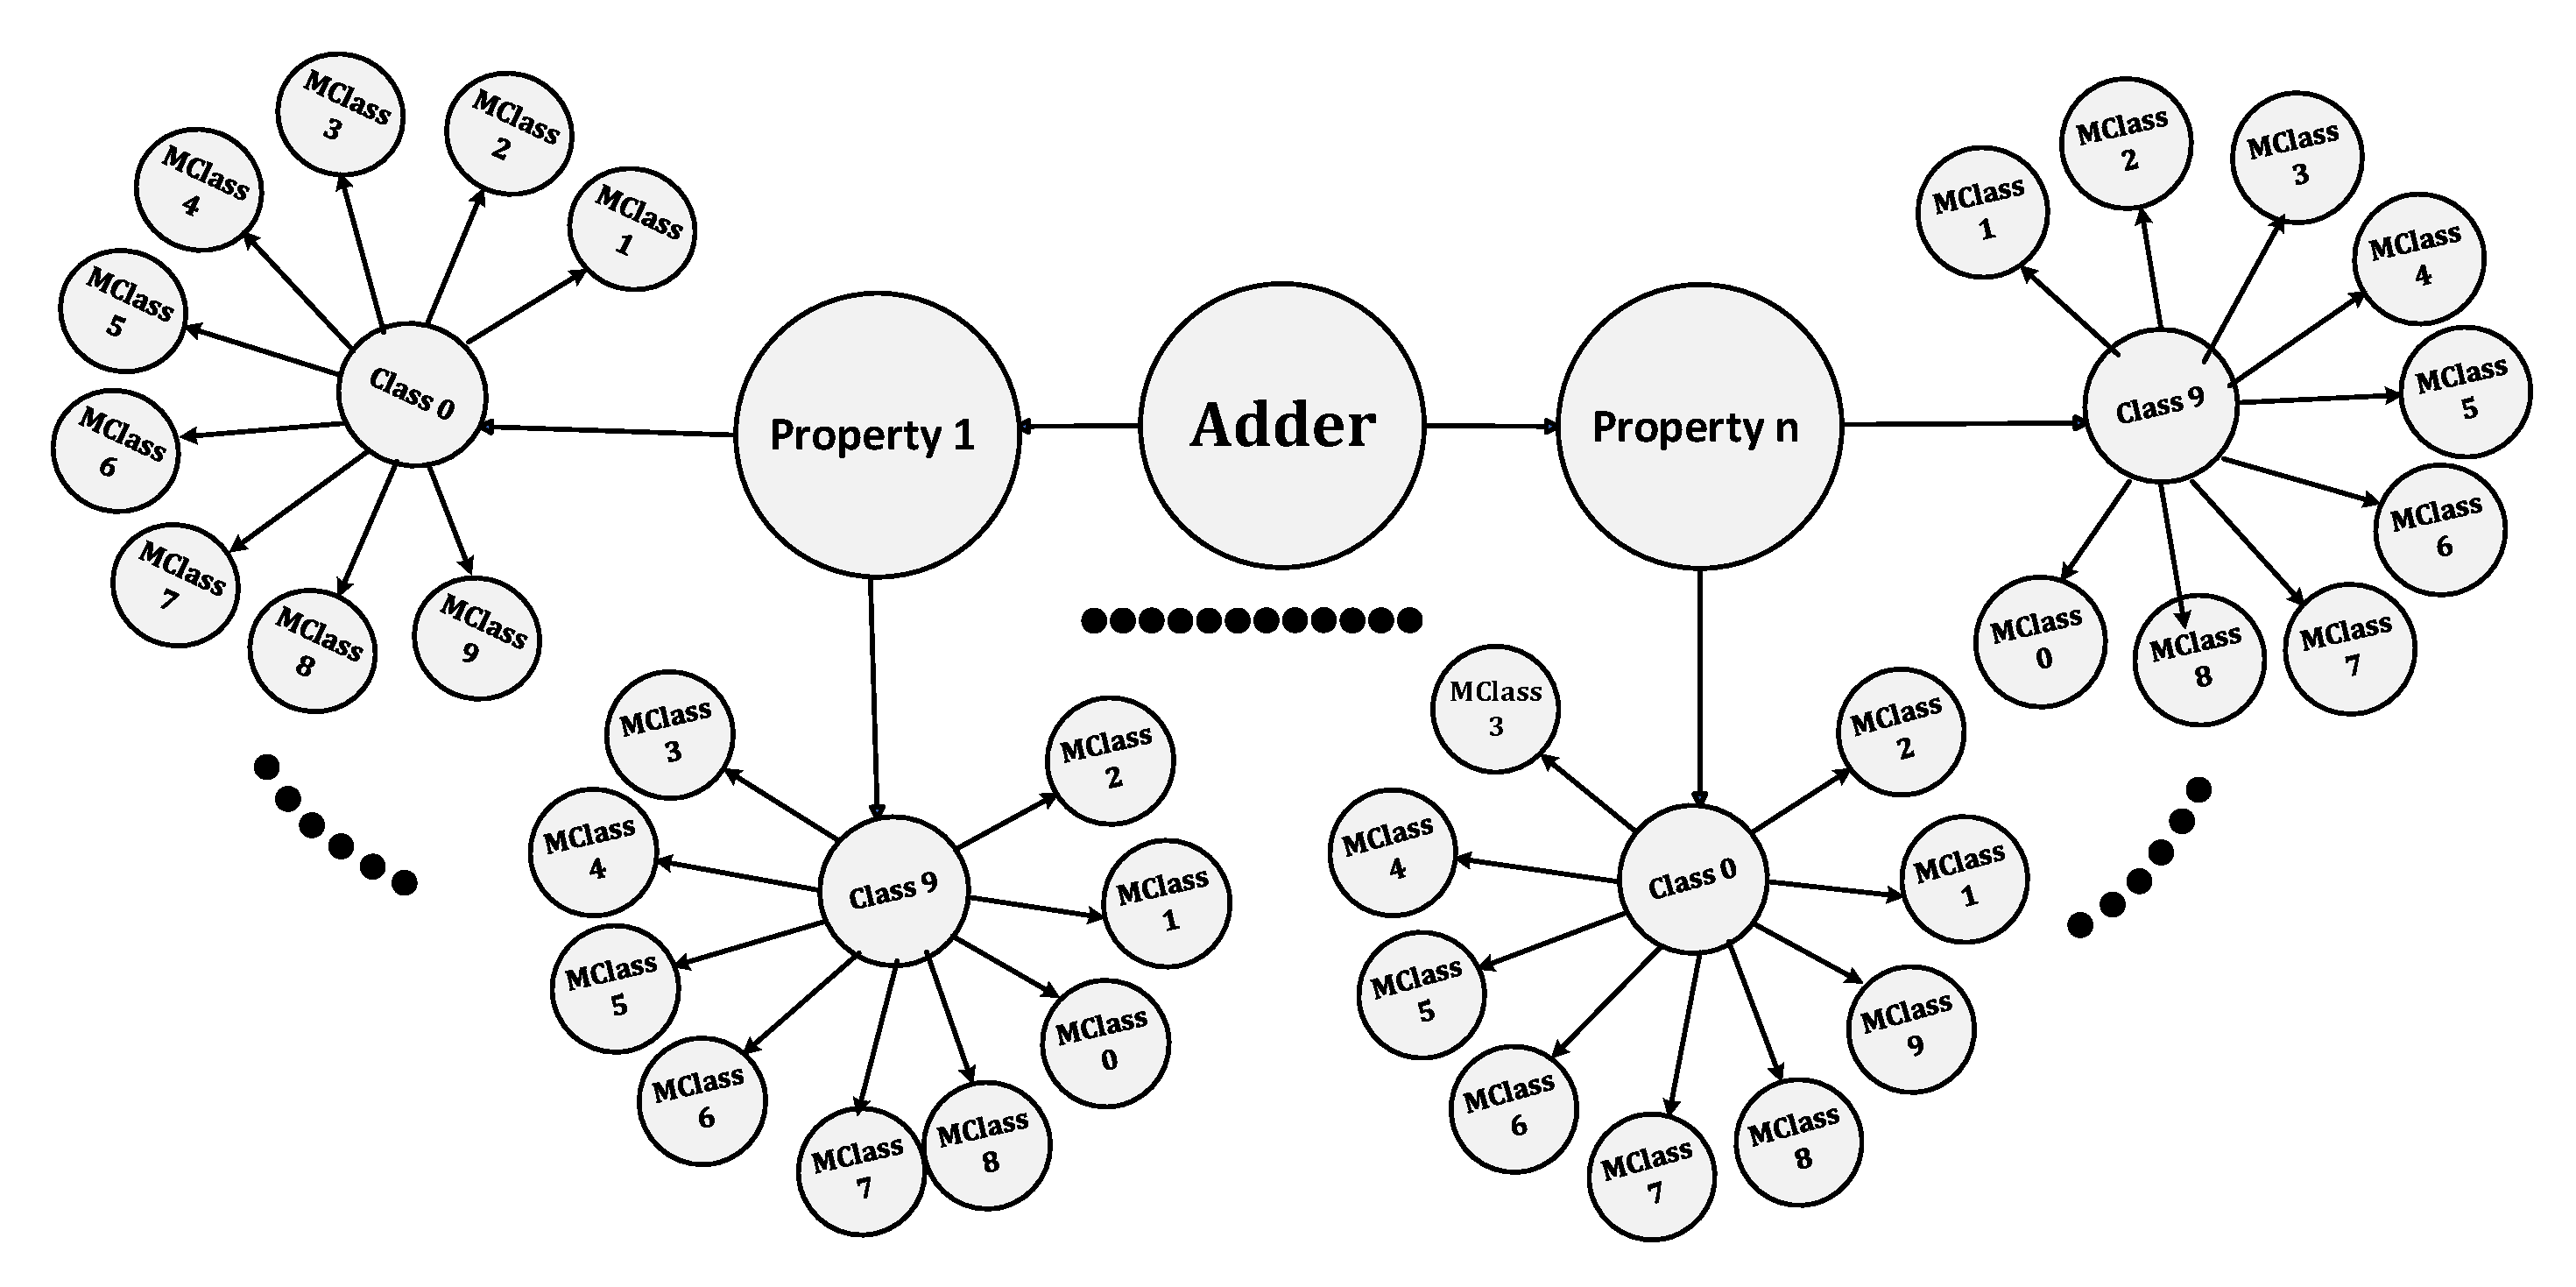
\includegraphics[width=\linewidth]{paper_images/step5.pdf}
    \caption{Diagram of Error Summarization Highlighting Class-Property Impact}
    \label{fig:error-summarization}
\end{figure}



\begin{enumerate}
    \item \textbf{Initial Error Detection:}
        The combined prediction incorrectly sums to `6' instead of `5'.

    \item \textbf{Identify the Inaccurate Predictions:}
        Examination reveals the model predicts `6' for Class A and correctly predicts `0' for Class B.

    \item \textbf{Drill Down to Property Level:}
        Both images were tested under noise. The noise robustness for each class is assessed:
        \begin{itemize}
            \item \( LR_{A,p_1} = 85\% \) — suggesting a 15\% failure rate.
            \item \( LR_{B,p_1} = 90\% \)
        \end{itemize}

    \item \textbf{Assess Individual Local Robustness:}
        Focus is placed on Class A's noise robustness, identifying potential misclassification trends under noisy conditions.

    \item \textbf{Further Analysis:}
        Investigate if certain noise patterns consistently mislead the model concerning digit `5', potentially confusing it with a similar appearance to `6'.

    \item \textbf{Systematic Error Identification:}
        Patterns of error involving Class A under noise are sought to determine if specific adjustments in model training or data handling can mitigate these issues.

    \item \textbf{Propose Adjustments:}
        Modifications to the training process or data augmentation strategies are suggested to enhance noise robustness, especially for digits with appearances similar to `5'.
\end{enumerate}





\section{Experiments}


\section{Threats to Validity}

This section outlines significant limitations and assumptions in our study that may affect the validity and reliability of our findings.

\begin{itemize}
    \item \textbf{Random Sampling:} Our current approach assumes a uniform distribution of samples across all classes, which may not represent the true complexity and variability within real-world data. This uniform sampling can lead to biased evaluations if the class distribution in practical applications is skewed or non-uniform. We plan to enhance our sampling techniques to better capture the diversity and distribution of data in realistic scenarios. Improved sampling strategies will help in developing more robust and generalizable error summarization methods.
\end{itemize}


\section{Related Work}
% Your content here

\section{Conclusion}
% Your conclusion here

\begin{thebibliography}{01}
    \bibitem{Saad} Reference details
\end{thebibliography}

\end{document}
